	\documentclass[../pfc.tex]{subfiles}
	
	\begin{document}
	
	\section{Plan de desarrollo de software}
	
	Para el desarrollo de este aplicativo se seguirán los principios del Agile Manifesto \cite{agile}, y de entre todas las metodologías que lo implementan utilizaremos Scrum, ya que nos permite desarrollar siempre sobre algo ejecutable y tiene una buena "pelea contra el tiempo" o "timeboxing" ya que al final de cada sprint hay que hacer una retrospectiva sobre lo que ya se ha construido y entregado.

	\section{Propósito general de la planificación}
	
	La planificación nos debe dar una cifra orientativa del esfuerzo a comprometer para acometer un desarrollo de un proyecto software. Pero debido a lo mencionado anteriormente sobre el manifiesto ágil, creemos que dar una cifra estimativa en tiempo es venturoso, más si queremos ceñirnos a el y más aún cuanto mas a largo plazo sea la estimación. Por eso las metodologías ágiles suelen ocultar la referencia temporal de los desarrollos y estiman la complejidad de las tareas, sabiendo por el histórico, ya que los equipos deben ser fijos en el tiempo, la complejidad aproximada que un equipo dedicado a un proyecto puede acometer. 
	
	\section{Metodología }
	
	Tradicionalmente se denomina metodología de desarrollo de software a un marco de referencia para estructurar, planificar, controlar y medir el proceso de desarrollo de software.\cite{wiki-metodologia}
	
	En los últimos años se han popularizado diversas metodologías que "rompen" en parte con los paradigmas anteriores a cambiar el punto sobre el que ponen el foco. Es en estas nuevas metodologías, que se han venido a denominar ágiles por su capacidad rápida de respuesta al cambio, donde vamos a encontrar la metodología que vamos a utilizar para el desarrollo del proyecto.
	
	Como generalidades sobre las metodologías ágiles decir que se basan todas ellas en la formación de grupos auto organizados y multidisdisciplinares que colaboran para llevar a cabo el proyecto. De hecho es esta colaboración y esta auto organización las piezas clave para que el equipo vea que tiene poder de decisión durante la vida del proyecto, y que de esta manera se implique mucho más en el éxito del mismo.
	
	Para la realización del proyecto buscaremos como ya hemos comentado dentro las diferentes metodologías ágiles, hemos elegido SCRUM, por ser la que mejor se adapta a la continua pelea contra el tiempo que el equipo debe mantener. \\
	Lo primero que debemos decir es que SCRUM es una metodología iterativa e incremental que promueve la auto organización de los equipos de desarrollo y un esquema de colaboración con el cliente, haciéndose responsable de que las prioridades, los requisitos, etc pueden cambiar por parte de este, y que es responsabilidad del propio equipo el asumir y responder a estos cambios. 
	
	\subsection{SCRUM}
	
	SCRUM como metodología fué propuesto por Ikujiro Nonaka e Hirotaka Takeuchi a principios de los 80, al analizar cómo desarrollaban los nuevos productos las principales empresas de manufactura tecnológica: Fuji-Xerox, Canon, Honda, Nec, Epson, Brother, 3M y Hewlett-Packard (Nonaka \& Takeuchi, The New New Product Development Game, 1986).\\
	Aunque esta forma de trabajo surgió en empresas de productos tecnológicos, es apropiada para proyectos con requisitos inestables y para los que requieren rapidez y flexibilidad, situaciones frecuentes en el desarrollo de determinados sistemas de software.\\
	
	SCRUM define un conjunto de prácticas y roles, que pueden tomarse como punto de partida para definir el proceso de desarrollo que se ejecutará durante un proyecto. Abordar un proyecto mediante SCRUM lleva a la repetición o iteración de la unidad básica del peoyecto denominada Sprint. Durante cada sprint, un periodo entre una y cuatro semanas (la magnitud es definida por el equipo y debe ser lo mas corta posible), el equipo crea un incremento de software potencialmente entregable (utilizable). El conjunto de características que forma parte de cada sprint viene del Product Backlog, que es un conjunto de requisitos de alto nivel priorizados que definen el trabajo a realizar a menudo denominadas Historias de usuario. Los elementos del Product Backlog que forman parte del sprint se determinan durante la reunión de Sprint Planning. Durante esta reunión, el Product Owner identifica los elementos del Product Backlog que quiere ver completados y los hace del conocimiento del equipo. Entonces, el equipo conversa con el Product Owner buscando claridad y magnitud adecuadas para luego determinar la cantidad de ese trabajo que puede comprometerse a completar durante el siguiente sprint. Durante el sprint, nadie puede cambiar el Sprint Backlog, lo que significa que los requisitos del sprint están congelados durante el propio sprint, pero podrían modificarse aquellos que aun estuviesen en el Product Backlog.\\
	
	SCRUM permite la creación de equipos autoorganizados impulsando la co-localización de todos los miembros del equipo, y la comunicación verbal entre todos los miembros y disciplinas involucrados en el proyecto, ya que una de la bases de SCRUM en la colaboración y comunicación entre todos los roles de un proyecto. \\
	
	Un principio clave de SCRUM es el reconocimiento de que durante un proyecto los clientes pueden cambiar de idea sobre lo que quieren y necesitan, y que los desafíos impredecibles no pueden ser fácilmente enfrentados de una forma predictiva y planificada. Por lo tanto, SCRUM adopta una aproximación pragmática, aceptando que el problema no puede ser completamente entendido o definido, y centrándose en maximizar la capacidad del equipo de entregar rápidamente y responder a requisitos emergentes.\\
	
	Las características más marcadas que se logran notar en SCRUM serían: gestión regular de las expectativas del cliente, resultados anticipados, flexibilidad y adaptación, retorno de inversión, mitigación de riesgos, productividad y calidad, alineamiento entre cliente y equipo, por último equipo motivado. Cada uno de estos puntos mencionados hacen que el SCRUM sea utilizado de manera regular en un conjunto de buenas prácticas para el trabajo en equipo y de esa manera obtener resultados posibles.\\
	
	Los beneficios para las empresas más notables al utilizar SCRUM son
	
	\begin{itemize} 
		\item Flexibilidad a cambios. Gran capacidad de reacción ante los cambiantes requerimientos generados por las necesidades del cliente o la evolución del mercado. El marco de trabajo está diseñado para adecuarse a las nuevas exigencias que implican proyectos complejos.
		Reducción del Time to Market. El cliente puede empezar a utilizar las características más importantes del proyecto antes de que esté completamente terminado. 
		\item Mayor calidad del software. El trabajo metódico y la necesidad de obtener una versión de trabajo funcional después de cada iteración, ayuda a la obtención de un software de alta calidad.
		Mayor productividad. Se logra, entre otras razones, debido a la eliminación de la burocracia y la motivación del equipo proporcionado por el hecho de que pueden estructurarse de manera autónoma.
		\item Maximiza el retorno de la inversión (ROI). Creación de software solamente con las prestaciones que contribuyen a un mayor valor de negocio gracias a la priorización por retorno de inversión.
		\item Predicciones de tiempos. A través de este marco de trabajo se conoce la velocidad media del equipo por sprint, con lo que es posible estimar de manera fácil cuando se podrá hacer uso de una determinada funcionalidad que todavía está en el Backlog.
		\item Reducción de riesgos El hecho de llevar a cabo las funcionalidades de mayor valor en primer lugar y de saber la velocidad a la que el equipo avanza en el proyecto, permite despejar riesgos efectivamente de manera anticipada
	\end{itemize}
	
	Como puntos flacos tanto de SCRUM como de muchas de las metodologías ágiles podemos observar:
	
		\begin{itemize} 
			\item Fuerte dependencia de las personas y en sus habilidades comunicativas y de auto organización
			\item Participación fuerte e intensa de todos los implicados en el proceso, con los riesgos por parte de unj cliente poco participativo
			\item Falta de documentación o mucha laxitud en la que existe.
		\end{itemize}
	
	Aunque más adelante en este documento se profundiza en la metodología aquí se muestra una imagen que puede servir como resumen de todos los conceptos roles y rituales de SCRUM.
	
		\begin{figure}[h]
			\centering
			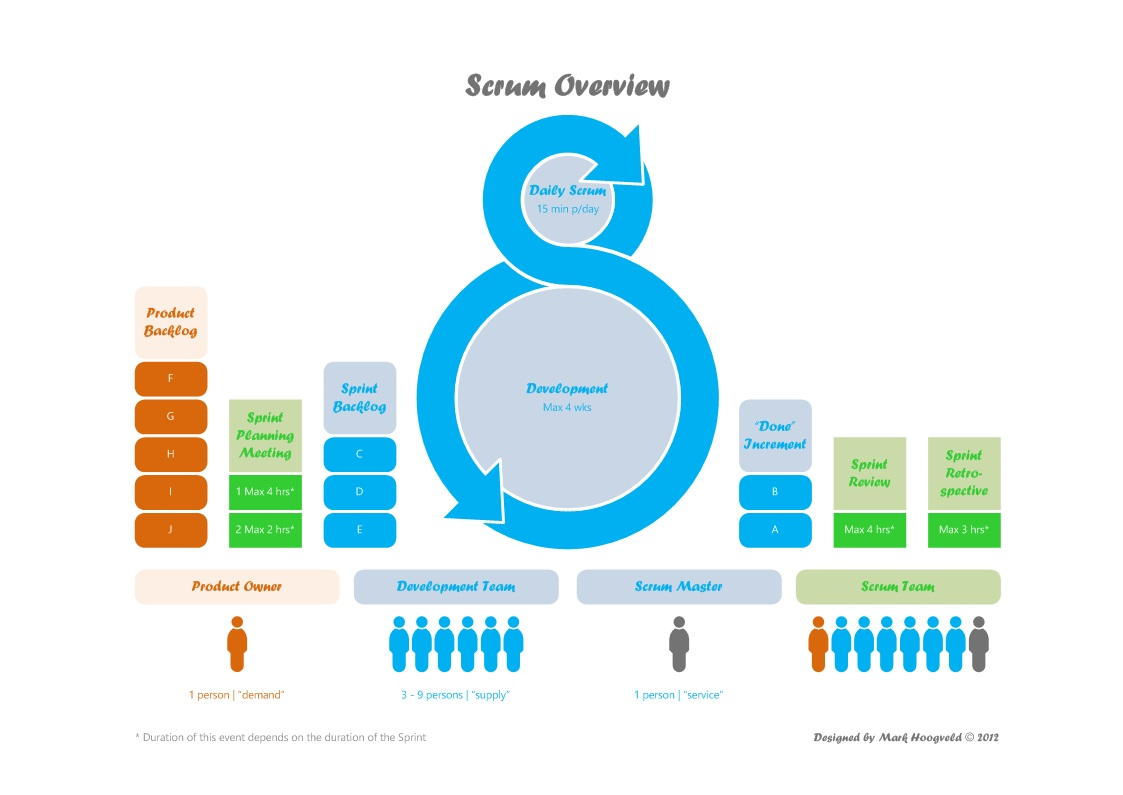
\includegraphics[max width=\textwidth]{scrum-overview}
			\caption{Resumen de Scrum.}
			\label{fig:Resumen de Scrum}
		\end{figure}
	
	\subsection{Roles y responsabilidades}
	Los roles  implicados en el proceso de desarrollo y sus responsabilidades   de la app son:

	\textbf{Product Owner}\\*
	El Product Owner representa la voz del cliente, que puede ser el cliente mismo o alguien en su nombre. Se asegura de que el equipo trabaje de forma adecuada desde la perspectiva del negocio. El Product Owner escribe historias de usuario, las prioriza, y las coloca en el Product Backlog, de hecho se suele decir que el Product Owner es el dueño del Product Backlog. E nuestro caso este rol lo llevaban a cabo varias personas con las que hemos tenido contacto en la AECC.\\
	
	\textbf{ScrumMaster (o Facilitador)}\\*
	El Scrum es facilitado por un ScrumMaster, cuyo trabajo primario es eliminar los obstáculos que impiden que el equipo alcance el objetivo del sprint. El ScrumMaster no es el líder del equipo (porque ellos se auto-organizan), sino que actúa como una protección entre el equipo y cualquier influencia que le distraiga. El ScrumMaster se asegura de que el proceso Scrum se utiliza como es debido. El ScrumMaster es el que hace que las reglas se cumplan. Quizá este es el puesto clave de Scrum ya que se encarga de que el equipo se centre en producir aquello que el Prodcut Owner ha marcado. En nuestro caso este rol ha sido una surte de Frankestein ya que para algunas tareas ha sido el personal de la AECC, para otras ha sido el tutor y en algún caso nosotros mismos saliendo del rol de equipo. \\
	
	\textbf{Equipo de desarrollo}\\*
	El equipo tiene la responsabilidad de entregar el producto. Es recomendable un pequeño equipo de 3 a 9 personas con las habilidades transversales necesarias para realizar el trabajo (análisis, diseño, desarrollo, pruebas, documentación, etc).\\
	
	A veces se definen más roles que pueden complementar en alguna fase a estos, o ayudar en tareas administrativas, pero formalmente quedan un poco fuera de la metodología por mas que sean muy necesarios en las empresas hoy día.
	
	\subsection{Eventos y rituales}
	
	Dentro de la metodología de SCRUM existen varias reuniones o rituales, tras las que se esconde alguno de los principios o practicas de las metodologías ágiles\cite{agile}, dentro de que cada equipo debe adaptar la metodología a su idisioncrasía y condiciones particulares, se recomienda en la medida de lo posible ajustarse a las mismas ya que que la ganancia que reportan está comprobado que refuerza todos los esfuerzos de la metodología. 
		
	\textbf{Sprint}\\* 
	No es en sí un evento o un ritual, simplemente es la medida de tiempo en los que se dividen los proyectos a acometer por el eqiupo. Así el Sprint es el período en el cual se lleva a cabo el trabajo en sí. Se recomienda que la duración de los sprints sea constante y definida por el equipo con base en su propia experiencia. Se puede comenzar con una duración de sprint en particular (2 o 3 semanas) e ir ajustándolo con base en el ritmo del equipo, aunque sin relajarlo demasiado. Al final de cada sprint, el equipo deberá presentar los avances logrados, y el resultado obtenido es un producto potencialmente entregable al cliente. Asimismo, se recomienda no agregar objetivos al sprint o sprint backlog a menos que la falta de estos objetivos amenace al éxito del proyecto. La constancia permite la concentración y mejora la productividad del equipo de trabajo.\\
	
	\textbf{Daily Scrum o Stand-up meeting}\\*
	Cada día de un sprint, se realiza la reunión sobre el estado de un proyecto. Esto se llama daily standup o Stand-up meeting. El scrum tiene unas guías específicas:
	\begin{itemize} 
		\item La reunión comienza puntualmente a su hora. 
		\item Todos son bienvenidos, pero sólo los involucrados en el proyecto pueden hablar. (Esto es el equipo y el scrum master). 
		\item La reunión tiene una duración fija de 15 minutos, de forma independiente del tamaño del equipo.
		\item La reunión debe ocurrir en la misma ubicación y a la misma hora todos los días.
		\item Durante la reunión, cada miembro del equipo contesta a tres preguntas:
		\begin{enumerate}
			\item ¿Qué has hecho desde ayer?
			\item ¿Qué es lo que harás para mañana?
			\item ¿Has tenido algún problema que te haya impedido alcanzar tu objetivo? (Es el papel del ScrumMaster recordar y anotar estos impedimentos para su posterior análisis y subsanación si procede).
		\end{enumerate} 
	\end{itemize}
	
	\textbf{Reunión de Planificación del Sprint }\\*
	Al inicio de cada ciclo de Sprint, se lleva a cabo una reunión de planificación del Sprint. en esta reunión debe estar el equipo al completo, el scrum master y el product owner Se pretende:
	\begin{itemize} 
		\item Seleccionar qué trabajo se llevará a cabo por el equipo durante el sprint 
		\item Preparar, con el equipo completo, el Sprint Backlog o sea las tareas del sprint clarificando el Product Owner las posibles dudas o  inconsistencias que el equipo detecte en la redacción de las tareas, este se debe extraer de las tareas más prioritarias del Product Backlog, de acuerdo con el Product Owner. 
		\item Identificar y comunicar cuánto del trabajo es probable que se realice durante el actual Sprint.
	\end{itemize}
	
	Realizarse esta planificación en ocho horas como tiempo límite.\\
	
	\textbf{Reunión de Revisión del Sprint}\\*
	Al finalizar cada sprint se organiza esta reunión en la que que el equipo presenta el trabajo desarrollado durante el sprint en lo que se denomina Incremento de Producto Potencialmente Entregable. Durante esta reunión tiene lugar la presentación del ejecutable en lo que se denomina Demo. Así pues las principales actividades de esta reunión serían:
	\begin{itemize} 
		\item Revisar el trabajo que fue completado y no completado 
		\item 	Presentar el trabajo completado a los interesados, entre ellos el product owner y que estos de su aprobación al mismo o presenten sus quejas o matices (alias “demo”), pero teniendo en cuenta que los estados del trabajo son binarios, está acabado o no está acabado, no hay porcentajes intermedios. 
		\item El trabajo incompleto no puede ser demostrado 
	\end{itemize}
	
	Para esta reunión y dependiendo del tamaño del sprint se dispondrá de cuatro horas como límite\\
	
	\textbf{Retrospectiva del Sprint }\\*
	Después de cada sprint, se lleva a cabo una retrospectiva del sprint, en la cual todos los miembros del equipo dejan sus impresiones sobre el sprint recién superado. El propósito de la retrospectiva es realizar una mejora continua del proceso. Esta reunión tiene un tiempo fijo de cuatro horas.
	
	\section{Planificación completa}
	
	Para realizar la planificación completa de la app debemos antes introducir algunos conceptos a la estimación en el contexto de las metodologías ágiles, como son velocidad del equipo, historias de usuario, puntos de historia, etc.    
	
	\subsection{Historias de Usuario e Historias Épicas}
	
	Los requisitos en la mayoría de las metodologías ágiles se condensan en lo que se viene a llamar historias de usuario. Formalmente hablando una historia de usuario es una representación de un requisito de software escrito en una o dos frases utilizando el lenguaje común del usuario o del negocio del usuario, esto es esencialmente NO técnico.Describe una funcionalidad que, por sí misma, aporta valor al usuario.\\
	
	El formato físico o registral de estas historias de usuario suelen ser tarjetas de papel/cartón con espacio para colocar post its de tareas asociadas a la historia, y estas pueden ser tan complejas o simples como el equipo, scrum master y product owner decidan entre ellos, pero como minimi deberían tener una descripcion del tipo como XXX quiero YYY para ZZZ y una estimación en puntos de historia. Pero no hay problema si se añaden un criterio de aceptación de la historia, una identificación de la misma, un título, etc\\
	
	Idealmente las historias de usuario deberían escribirse por el product owner, pero más idealmente aún es si se escriben en conjunto y conversando sobre el aporte de la misma al producto final. En el sprint planning se decide cuales de las historias más arriba en la pila del product backlog entraran a realizarse en este sprint, clarificando el product owner las dudas que sobre las mismas puedan surgir al equipo.
	
	La siguiente figura muestra lo que podría ser una tipica tarjeta de historia de usuario, con los datos más importantes y alguno que en esa organización tenga sentido, pues recordamos que Scrum son guías y que cada equipo debe enocntrar la manera de adaptarse lo mejor posible a la matodología pero tambien de adaptar esta a unas fomras en las que se sientan cómodos. \\ 
	
	\begin{figure}[h]
		\centering
		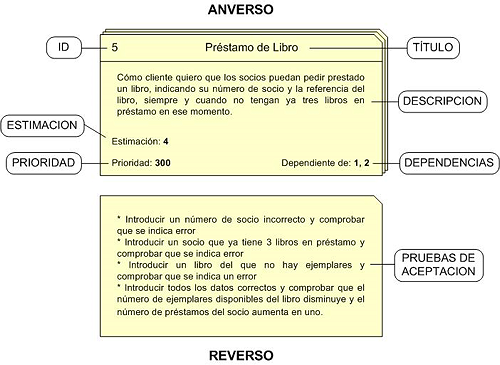
\includegraphics[max width=\textwidth]{historia}
		\caption{Ejemplo de historia de usuario}
		\label{fig:ejemplo de historia de usuario}
	\end{figure}
	
	\subsection{Puntos de Historia}
	
	Los puntos de historia son una medida de la complejidad de la tarea a abordar. Se utilizan para evitar dterminados efectos asoaciados a estimar en tiempo y que repertcuten en baja calidad de código y tensiones innecesarias en el equipo. De esta manera el equipo fija una historia de usuario tipo y conocida con una medida arbitraria de puntos de historia, y el resto de historias se evaluan en tornoa esa misma, de tal manera que si por ejemplo a nuestra historia de usuario modelo le fijamos una media de puntos de historia de 3, si después tenemos una historia que tiene el doble de complejidad, deberiamos estimarla en 6.\\
	
	A este respecto decir que para estimar la complejidad de las historias existen varias maneras, pero una de las más usadas el planning poker, consistente en que todos los miembros del equipo establecen en secreto un valor de puntos de historia después de que la historia sea leida y en su caso aclarada. Estos valores no son libres y suelen estar relacionados con valores similares a la serie de Fibonacci (1, 2, 3, 5, 8, 13, 20). Si existe discrepancia entre miembros del equipo el scrum master puede conminarles a que expliquen los motivos por los que asignan dicho valor, tras lo cual se repetira la votación. Esto se hace así para poner de relieve complejidad oculta que nadie ha detectado o viceversa.
	
	\subsection{Velocidad de un equipo}
	
	El concepto de velocidad del equipo es la cantidad de puntos de historia que se acomenten en un sprint. Es un valor que depende de la experiencia pasada del equipo y que suele calcularse manteniendo un registro historico de los puntos resueltos por el equipo en los anteriores sprints. Es una medida que depende de que el equipo sea una unidad más o menos constante a lo largo del tiempo. 
	
	\subsection{Planificación de los Sprints}   
	
	Teniendo en cuenta las historias de usuario, desglosdas y tratadas con más detalle en el capitulo siguiente, y la estimacion de estas que podemos ver en el listado posterior, vemos que el total de puntos de historia del proyecto puramente tecnico son XXX, haciendo un pr de sprints inciales de setup de proyecto y de abordamiento de tareas muy generales y las primeras historias de usuario, obtuvimos que la velocidad del equipo era YYY, valor que se modificó posteriormente a YYY' al final del proyecto, por tanto estimamos que fueron ZZZ sprints que al termino del proyecto con sprints de deuda tecnica y de resolucion de algun error se quedo en ZZZ' lo cual no se habia alejado en exceso de la estimación inicial. 
	
	Decir que en los contratos propios de Scrum, lo que suele hacerse es hacer ua estimación del proyecto inicial y contratar al equipo por un numero de sprints suficientes para el desarrollo del mismo. Pudiendose despues alargar estos sprints o acortarse si se consigue el exito con antelación. En este tipo de contratos lo que suele hacerse es contratar un tiempo determinado y en ese mismo tiempo decidir que funcionalidades implementar, pudiendose cortar el proyecto al termino de un sprint si el product owner considera que el producto tiene la suficiente madurez, o por contra modificar, ampliar o repensar esas funcionalidades en sprints hasta que se considere que tiene lo que desea. 
	
	
	\section{Recursos necesarios}
	Los recursos designados para la realización completa de este proyecto serán los siguientes:\\
	
	\textbf{Recursos humanos}
	
	\begin{itemize} 
		\item El equipo, en este caso los alumnos que defienden este proyecto. 
		\item El scrum master, como se ha mencionado este papel esta repartido entre el tutor, personas involucradas desde la AAEC y en ocasiones alguno de los alumnos. 
		\item El product owner, que ya se ha dicho antes en este documento son varias personas dentro de la AECC. 
	\end{itemize}
	
	Determinar el esfuerzo del rol equipo en este proyecto es sencillo, pero el resto deroles es más complejo el computar las horas de dedicación a este proyecto de cara a realizar una planificacion, de tal manera que se estimará que el rol scrum master sea un 30\% del tiempo consumido por el equipo y por contra el rol de product owner se estimará en un 25\% de la anterior medida.\\\\
	
	\textbf{Recursos Software}
	
	Los recursos software para esta iteración serán:
	\begin{itemize}
		\item Microsoft Project 2003 como herramienta de planificación
		\item TexStudio + Sharelatex herramienta de elaboración de documentos PDF
		\item Adobe Photoshop CS6 para realizar ilustraciones e imágenes
		\item StarUML y Enterprise Architect para modelado y diagramas
		\item Dropbox y github como herramientas para compartir código y archivos
		\item Android Studio como IDE (Integrated Development Enviroment o entorno integrado de desarrollo) para el desarrollo del código Android necesario
		\item SQLLite como sitema gestor de bases de datos en el dispositivo móvil\\\\
	\end{itemize}
	
	\textbf{Recursos Hardware}
	
	Los recursos hardware para esta iteración serán:
	
	\begin{itemize}
		\item Dos ordenadores portátiles personales
		\item Un ordenador Personal de sobremesa
		\item Varios móviles con SO Android
		\item Memoria USB para el intercambio de datos
		\item Cables USB - Micro USB (Debug)
	\end{itemize}	
	
\end{document}